%!TEX root=../thesis.tex
\chapter{A Real-Time model for WebGL} \label{cha:rt_model}

WebGL is a relatively new technology that enables hardware-accelerated web
contents. Moreover, in the last few years Virtual Reality (VR) has became
another very popular research topic. The Mozilla Foundation is actively working
for porting VR technologies to the Web my means of WebVR~\cite{mozvr}. WebVR is
``an open specification that makes it possible to experience VR'' inside a web
browser, whose main goal is to make VR experiences easier regardless of the
device used. This specification~\cite{webvrspecs} is made available to developers
through different frameworks such as Mozilla's A-Frame~\cite{aframe}, which allows
to build virtual reality scenes inside the browser using only HTML and JavaScript
code. This may seem a very different approach with respect to the one of this
thesis, but what makes A-Frame similar to Cesium is how they exploit WebGL to
interact with the GPU to achieve hardware acceleration. In this sense it is
reasonable to compare VR and 3D map web technologies since they both use WebGL
as its core part. Furthermore, virtual reality applications are even more
performance-demanding, since large latencies jeopardize the entire user
experience.


\section{Assumptions}
First of all, all the experiments presented in this thesis are run on a Dell
Inspiron 15R 5521 notebook\footnote{\url{http://www.dell.com/us/dfh/p/inspiron-15r-5521/pd}.},
whose hardware specifications are shown in Table \ref{tab:notebook_specs}.
Since graphics performances highly depends on the GPU available to the system,
the results presented in Chapter \ref{cha:experiments} are likely to be overtaken
if better graphics hardware (eg. a dedicated GPU) is installed.
\begin{table}[!htb]
    \centering
    \caption{The test machine hardware specifications.}
    \label{tab:notebook_specs}
    \begin{tabular}{|l|l|l|l|}
    \hline
    \multicolumn{1}{|l|}{\textbf{CPU}} & \multicolumn{1}{l|}{\textbf{GPU (integrated)}} & \multicolumn{1}{l|}{\textbf{RAM}} & \multicolumn{1}{l|}{\textbf{Hard drive}} \\ \hline
    Intel i7 3537U & Intel® HD Graphics 4000 & 8GB DDR3 & Samsung 850 Evo 250GB \\ \hline
    \end{tabular}
\end{table}

Another important aspect is how tests are conceived. As it is always the case in
real-time analysis, the worst possible scenario is the interesting one for
computing the WCET of a task. To achieve this situation using the test application,
Google Chrome is always run from scratch with only one active tab. Moreover, the browser
is forced not to cache any part of the application code but, at the same time, it
is essential to get rid of the map tils' retrival time. Usually map tiles are
downloaded via HTTP using the REST APIs a terrain server exposes to the clients.
Even the time the navigator takes to download a small portion of the terrain
can be orders of magniture bigger than all the rest of the response time.
Hence, this particular task is obtained allowing the browser to save locally the
tiles downloaded during a ``warm-up'' phase. This allows to significantly lower
the map retrival time during the ``real'' experiment that is later discarded from
the trace.

Finally, picking timestamps during the execution of a piece of software can bias
the correctness of the timings themselves. This is another point that has to be
taken into account during any type of analysis involving time measurements like
the one presented in this work. In simple terms, measuring time takes time.


\section{Tools used}
This section presents the tools used to trace function calls and to pick the needed
timings in the experiments (see Chapter \ref{cha:experiments}).

\subsection{Web Tracing Framework}
The Web Tracing Framwork~\cite{wtf} (WTF) is composed of a set of tools for
instrumenting, analyzing and visualizing web application execution traces.
It is an extensible framework able to capture and replay HTML5 canvas elements
with its WebGL content. In this way it is possible to implement a plugin for WTF
for the specific purpost of the application under test. Furthermore, a wide set
of methods and events can be tracked out-of-the-box for preliminar investigations.

WTF is a very good toolset for an high-level analysis of web applications,
providing easy code instrumentation to track only what is truly interesting.
The usual work-flow is the following. First, the developer either selects the events
to be traced from a predefined set or he/she implements its own specific code
instrumentation with the available APIs. After that, the application's source code
has to include three function calls to prepare, start and stop tracing.
An example of application source code is the following:
\begin{lstlisting}[caption=Usage example of the Web Tracing Framework., language=JavaScript,
  label=code:wtf_example]
  let wtfOptions = { ... }; // customize WTF behaviour
  wtf.trace.prepare(wtfOptions);
  /* application initialization */
  wtf.trace.start(); // start profiling
  /* code to be traced goes here */
  wtf.trace.snapshot("file://trace"); // save trace to file
  wtf.trace.stop(); // stop profiling
\end{lstlisting}

After taking a snapshot of the current trace (line 6) and WTF is stopped (line 7,
code snippet \ref{code:wtf_example}), the trace is exported in a
compressed format that can be manipulated using some CLI
scripts\footnote{\url{https://github.com/google/tracing-framework}.} to export
data in Comma Separated Values (CSV) format or it can be visualized inside a web
page\footnote{\url{http://google.github.io/tracing-framework/bin/app/maindisplay.html}.}.

Another highlight is its extendibility. In this way, the developer can either
profile the application using events emitted by the browser by default or the
source code can be instrumented to track very specific parts. Basically, this
allows to measure nearly everything that is accessible from JavaScript, even
though it may not be enough in some situation.

Finally, there a post-process task is required in order to be able to get
insights from the CSV file. The format exported by the Web Tracing Framweork
is the following:
\begin{equation*}
    <time,\,value,\,total\_time,\,own\_time,\,arguments>
\end{equation*}

where:
\begin{itemize}
    \item \emph{time}: it is the amount of time (in milliseconds) elapsed from the
        \emph{wtf.trace.start()} function call.
    \item \emph{value}: it is the function name. More specifically this value is a
        string composed by\\
        ''\([context\_name]\#[function\_name]\)''.
    \item \emph{total\_time}: it is the time taken to complete the current invocation
        of the function (in milliseconds) along with any other function that
        is called.
    \item \emph{own\_time}: it is how long it took to complete the current invocation
        of the function (in milliseconds) not including any function called by
        the current one.
    \item \emph{arguments}: they are the actual arguments that are passed to the
        \emph{value} function.
\end{itemize}

Clearly, being the computaton of latencies the main aim this framework, the most
relevant fields for the analysis step are the \emph{time}, the \emph{total\_time}
and the \emph{own\_time}.


\subsection{Chrome's trace event profiler}
The other foundamental tool used to trace the navigator application is the trace
event profiler embedded into Google Chrome. This is another important reason why
Chrome is used as default browser for the entire work, since it allows to diagnose
performance issues and see what Chrome is really doing ``under the surface''.
This tool is available by default in any build of Google Chrome typing
\emph{chrome://tracing} inside the main URL bar.

This profiler ``records all the C++ and JavaScript method signatures in a
hierarchical view for each thread in each process'' of the browser. This results
in a huge amount of information, but it helps to identify performance bottlenecks
and all the events happening inside the browser instance. This tool allows to
better analyze a web application, collecting all the events occuring when the
application is running starting from the renderer processes IPC up to every single
function that is executed by the GPU process. Sometimes it may be necessary
to run Chrome with some particular command line flag in order to enable the
``debugging mode'' for some feature. For example, the \emph{--enable-skia-benchmarking}
flag is needed for profiling the Skia graphics engine. These additional flags
are not enabled by default since users do not need to profile the entire browser
all the time and thus, skipping some instruction inside the browser's source code
can result in better response times and navigation speed. Hence it is possible
to say that this event profiler perfectly fits a low-level analysis of everything
that happens inside the complex architechture of Google Chrome.
As it is possible to see from Figure \ref{img:chrome_event_profiler}, this tool
is capable both to acquire data from the browser and to visualize them as flame
graphs~\cite{gregg2016flame}.
\begin{figure}[!htb]
    \center{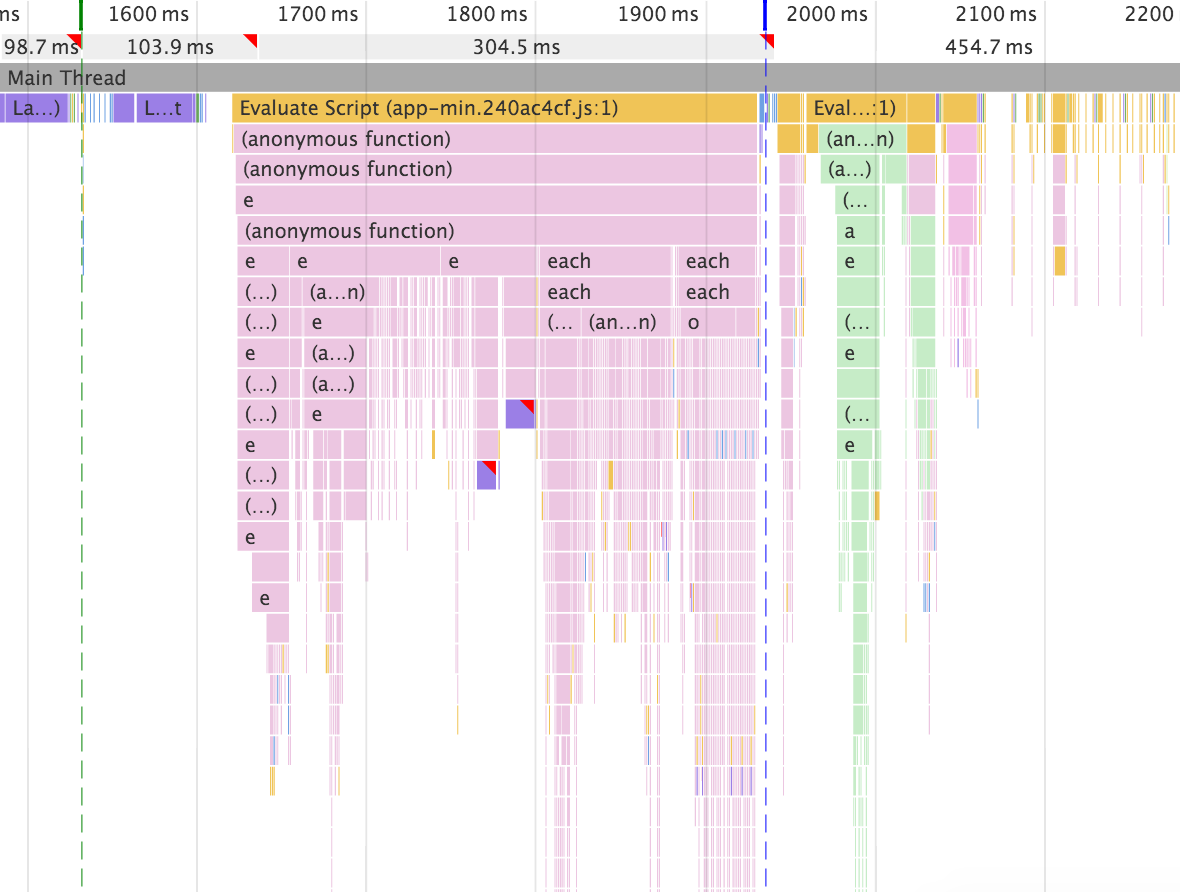
\includegraphics[width=0.55\linewidth]{chrome_event_profiler.png}}
    \caption{The viewer user interface for the Chrome event profiler.}
    \label{img:chrome_event_profiler}
\end{figure}

The output format of this tool is JavaScript Object Notation (JSON) file with a
lot of fieds. The ones of interest are the following:
\begin{lstlisting}
{
  "pid": 5782,
  "tid": 5782,
  "ts": 3951728304,
  "ph": "X",
  "cat": "gpu",
  "name": "GpuCommandBufferStub::OnAsyncFlush",
  "args": {
      "put_offset": 8958
  },
  "dur": 113,
  "tdur": 112,
  "tts": 1213475
}
\end{lstlisting}

where:
\begin{itemize}
    \item \emph{pid}: it is the process id of the process outputting the event.
    \item \emph{tid}: it is the thread id for the thread outputting the event.
    \item \emph{ts}: it is the tracing clock timestamp (in microseconds), meaning
        the amount of time elapsed from the tracing start.
    \item \emph{ph}: it is the event type that is recorded. This is a single character
        that depends on the type of event being tracked\footnote{A complete list
        of the type of events available can be found at the following link:
        \url{https://docs.google.com/document/d/1CvAClvFfyA5R-PhYUmn5OOQtYMH4h6I0nSsKchNAySU/}.}
    \item \emph{cat}: it represents the event category. This a list used to hide
        events from the Trace Viewer user interface.
    \item \emph{name}: it is the name of the event.
    \item \emph{args}: this contains any argument that is provided to the event/function
        call.
    \item \emph{dur}: it specifies the tracing clock duration of complete events
        (in microseconds).
    \item \emph{tdur}: it specifies the thread clock duration of complete events
        (in microseconds).
    \item \emph{tts}: it specifies the thread clock timestamp of the event (in
        microseconds).
\end{itemize}

The most important ones during the experiments are the \emph{ts} and the
\emph{tdur}, since they allow to define when an event has been fired and for how
much time the thread computing that function run.


\section{Profiling and analysis procedures}
There is some extra work to be explained which is a very convenient way to be able
to capture data with the tool presented in the previous section. There is a script
that simulates the FriWalk hardware sending its position and rotation to the web
interface via the WebSocket protocol. This is useful to simulate the behaviour of
a portion of the system architechture (see Figure \ref{img:system_arch}) that was
not always available during the development of this thesis.

Even from the very first test with WTF it became clear that the system under
test is as complex as the problem this thesis aims to solve. Therefore, the hard
problem of profiling the entire navigator application is split into many simpler
parts. Moreover, the navigator is traced from the startup of the application
until the first new position is sent by the FriWalk. This idea of reducing the
amount of workload to the minimum allows to better concentrate on fewer and more
specific data outputted by the tracing tools. Hence, the tests have been run in
four different scenarios:
\begin{itemize}
    \item the complete navigator application.
    \item a ``camera-only'' mode; in this scenario there is no physical placeholder
        to be moved on the map and only the user's camera is moved.
    \item a ``no-map'' mode; in this scenario the terrain map is completely
        excluded from the application. This means that no tail for the terrain is
        downloaded.
    \item a ``redraw'' mode; this is a scenario simulating a walker that remains
        stationary in the same position.
\end{itemize}

Every one of the scenarios mentioned above aims at simplifying the post-processing
analysis and to focus on the different parts of the navigator. For example, the
``no-map'' mode is conceived to get rid of the map but, at the same time, to keep
all the base functionalities of the navigator. To some extent, the partial traces
obtained from all these scenarios are necessary to compare each other and see their
similarities and their differencies.

Finally, a Python script is used in order to split and to graphically display the
timings extracted from the traces in a more effective manner.
